\section{Existing Solutions}

% EXISTING SOLUTIONS
% existing solutions

% intro

Three systems will be discussed in this area, each one 
withstanding common goals with the idealized solution.

ARVIKA is the biggest project so far in the
Augmented Reality domain. It offers a working solution to aid in industrial tasks but leaves most
of the regular user interfaces intact, leaving space for improvements at this level.
Additionally, it lacks an authoring tool to provide end-users means to set up scenarios in a friendlier manner.

Speech and Gestures shows a project where the Google Earth \cite{SITE-EARTH} application
-- a single user system that allows navigation in a world representation -- has been adapted to
work on a multi-touch surface with speech recognition.
The adapting work provided feedback about the limitations such software faces 
and offers a working solution to map most Google Earth actions to speech and gesture commands.

Finally, Digital Whiteboard provides a solution for multi-user digital
whiteboards where each user handles a palmtop serving as both the user's palette and
private composing area, supporting text and drawings input.
A technique called pick-and-drop is then explained. It is used to allow a user to transfer
the contents of the palmtop on the shared whiteboard.

\TODOL{SEE NEWEST ARTICLE REPOSITORY, NAMELY instant architecture and IPCity}


\subsection{ARVIKA, 2003}

ARVIKA \cite{ARVIKA} is a project with sponsoring from the
German Federal Ministry of Education and Research that was implemented between 1999 and 2003.
It focused on the development of Augmented Reality (AR) technologies to aid in performing industrial tasks.
The consortium involved several industrial partners such as Volkswagen, BMW, Siemens and Airbus.

\begin{figure}[!ht]
    \centering
    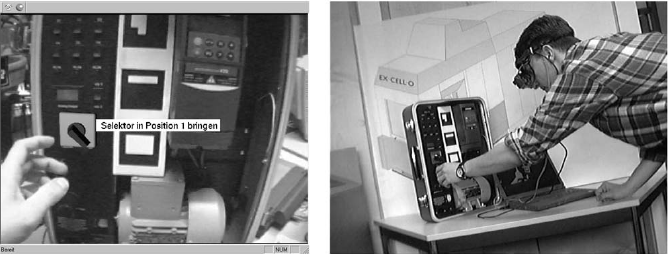
\includegraphics[width=10cm]{gfx/arvika.png}
    \caption{The augmented view seen from the HMD; a user of the ARVIKA system}
    \label{FIG-ARVIKA}
\end{figure}

An expert in the industrial area would carry a head-mounted display (HMD) with a camera mounted on it.
The real-time captured video was then interpreted and markers extracted from the image.
The camera's positioning and orientation were estimated and the HMD view was enriched with virtual objects
(see figure \ref{FIG-ARVIKA}, left).
The framework was distributed in the form of an ActiveX plug-in for the Internet Explorer browser
named ARBrowser.

% discussion

Weidenhausen et al. \cite{ARVIKA-LESSONS} consider the deployment of the project as an ActiveX component
to be an advantage since it is based on a widespread program (Internet Explorer) and allowed developers
to create task scenarios with familiar technologies such as JavaScript and HTML.
Although the world's largest research project in the area, ARVIKA focused too much on the technical problems
regarding AR and little effort was spent on the creation of a suitable user interface.
The authors agree on a point: ``most people judge the usefulness of a technology mainly by its user interface''.
Therefore this particular topic became work for future project iterations.
ARVIKA was meant to support many industrial scenarios -- development, production and services for several
industrial partners on different domains.
Creating a scenario was a time consuming task -- taking several days, according to Weidenhausen et al.
-- and required extensive knowledge in 3D modeling tools and VRML. No authoring capabilities were given to end-users.
This problem was identified as paramount and an authoring tool was scheduled for future development,
supporting generic task creation with parameters controlled by the users.



\subsection{Speech and Gestures on a Multi-User Tabletop, 2006}

Tse et al. \cite{SP-GEST-TTOP} developed a multimodal interface on top of Google Earth \cite{SITE-EARTH}
to be run on a multi-touch table.
The system allows multi-user collaboration with touch and voice commands.

The main problems found in adapting Google Earth reside in the fact that it was thought out as a single user program,
where only one action could be done at a time.
In this scenario several users could be disposed around the table with different orientations,
so text readability problems arose.
Additionally, user interface components such as the compass were placed at fixed points on the screen,
an approach that does not favor multi-user scenarios.
At 1024 x 768 resolution it was estimated that 42\% of the screen was originally consumed by GUI elements.
Since all users shared the surface, turn-taking had to be agreed by the users,
not being enforced by the system (see figure \ref{FIG-SP-TABLETOP}).
Most Google Earth interactive actions were mapped into gestures,
leaving the most abstract actions for voice commands activation (see figure \ref{FIG-SP-TABLETOP2}).


\begin{figure}[!ht]
    \centering
    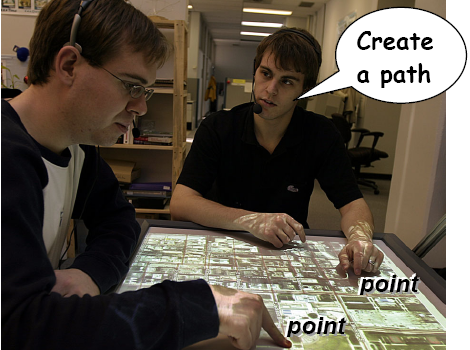
\includegraphics[width=7cm]{gfx/sp-gest-ttop.png}
    \caption{Two users collaborating on a Google Earth tabletop session}
    \label{FIG-SP-TABLETOP}
\end{figure}

\begin{figure}[!ht]
    \centering
    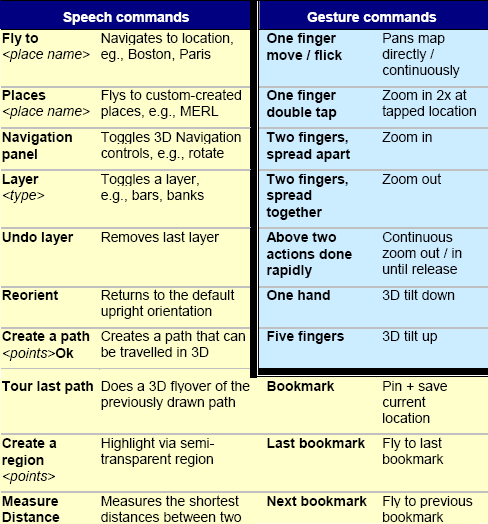
\includegraphics[width=8cm]{gfx/sp-gest-ttop2.png}
    \caption{The suggested speech and gesture interface for Google Earth}
    \label{FIG-SP-TABLETOP2}
\end{figure}

%\paragraph{Discussion}

This project shows the difficulties in adapting a production software thought out
for single user WIMP\footnote{Window Icon Menu Pointing device} interfaces for the support of collaborative scenarios.
A multimodal interface was built over the existing one, mapping most of its commands.
The set of obtained commands is a good example of how navigation can be performed on
3D scenery using a multimodal interface.
Google Earth is a good example of a navigation system suited for single user interaction.
It provides several functionality and could support the creation of buildings.
Making use of its large dataset of satellite images and topography would be excellent
for the target system.


\subsection{Digital Whiteboard, 1998}

Rekimoto \cite{WBOARD} presents a digital whiteboard where each participant is given
a palmtop computer to handle. It works as a tool palette, remote commander, text entry box as
well as a temporary data buffer during whiteboard collaboration interaction.

\begin{figure}[!ht]
	\centering
	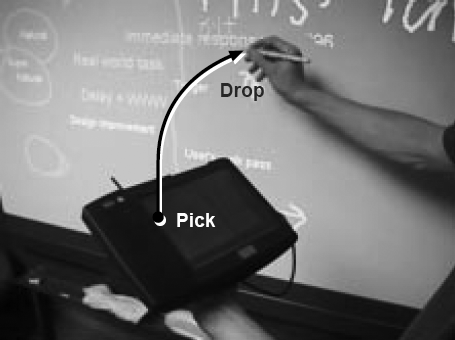
\includegraphics[width=6cm]{gfx/wboard.png}
	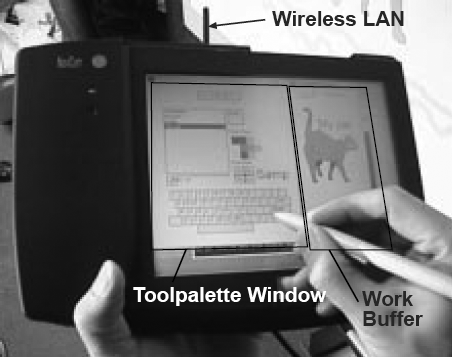
\includegraphics[width=6cm]{gfx/wboard2.png}
	\caption{Digital Whiteboard:
		Pick-and-drop interaction;
		Working areas for each participant's palmtop.}
	\label{FIG-WBOARD}
\end{figure}

The solution involves each participant carrying a pen and a palmtop,
with the pen working on both palmtop and whiteboard.
A direct manipulation method called Pick-and-drop(see Fig. \ref{FIG-WBOARD} left) was developed.
It allows a user to pick an object in his palmtop and dropping it on the whiteboard.
From the implementation point of view data is transferred through the network,
but from the user's perspective this technique allows him to pick up digital data
as if it were a physical object.
Text entry is performed on the palmtop and each user can choose the method he favors
(i.e.: handwritten recognition, soft keyboard, etc) for entering text.
No menus or tool palettes exist on the whiteboard -- they're available on each user's palmtop.
The main window is a multi page tool panel.
A user can flip to several tool palette pages, with the remaining area available as a temporary work buffer.
Users can store data elements in this window and paste them to the whiteboard
using Pick-and-Drop operations. (see Fig. \ref{FIG-WBOARD} right).

Rekimoto concludes that by putting many functions on palmtops,
users tend to concentrate too much on their own palmtop devices,
degrading mutual awareness among the participants.
Pick-and-Drop often worked better than drag-and-drop,
particularly when user had to move objects for a long distance.
Drag-and-drop forces a user to keep the pen tip in contact
with the board during the entire operation,
a restriction not suitable for large display surfaces.

%\paragraph{Discussion}

The solution where each user carries a palmtop for the creation of content such as note taking
is suitable for an architectural design and review scenario.
It grants the user the power to draw, type text or compose graphics 
independently from one another and then replicating the information on the whiteboard.
On the other hand there's the danger of users focusing too much on their paltop and losing
awareness of what's happening at the whiteboard.
